\documentclass[11pt, oneside]{article}
\usepackage{geometry}
\geometry{letterpaper}
\usepackage{graphicx}
\usepackage{amssymb,amsmath,parskip}
\usepackage{array}
\usepackage{longtable}

\newcommand{\tabitem}{~~\llap{\textbullet}~~}
\newcolumntype{L}[1]{>{\raggedright\let\newline\\\arraybackslash\hspace{0pt}}m{#1}}
\newcolumntype{C}[1]{>{\centering\let\newline\\\arraybackslash\hspace{0pt}}m{#1}}
\newcolumntype{R}[1]{>{\raggedleft\let\newline\\\arraybackslash\hspace{0pt}}m{#1}}

\title{SE350 Operating Systems Documentation}
\author{Gaisano, G., Janecka, L., Mak, R., Schneider, C.}


\begin{document}
\maketitle

\section{Introduction}
The following documentation details the implementation of a operating system written for the University of Waterloo SE350 course. The OS contains basic memory management, basic process handling, and essential system processes.

This documentation will cover:
\begin{itemize}
\item Global variable documentation;
\item Kernel API;
\item Interrupts and their handlers/processes;
\item System and user processes;
\item Initialization;
\item Testing;
\item Major design changes; and,
\item Timing analysis
\end{itemize}

\clearpage
\section{Global Variable Documentation}
Everyone
\begin{itemize}
\item What does each variable store?
\item Why is there a variable to store this?
\item What do your global data structures look like?
\item What functions use it?
\end{itemize}

{\bf Global Variables}
\begin{description}
\item [VARIABLE\_NAME] Stores x for y purpose, used by:
\begin{itemize}
\item z
\end{itemize}
\end{description}

{\bf Global Data Structures}
\begin{description}
\item [DATA\_STRUCTURE\_NAME] Stores x for y purpose, used by:
\newline
\begin{longtable}{|L{2cm}|L{5cm}|L{5cm}|} \hline
\textbf{Structure Name} & \textbf{Purpose} & \textbf{Properties} \\ \hline
Queue& generic queue &
\tabitem \textbf{Element *first}: pointer to first element in the Queue. Is NULL if there are no elements.
\newline
\tabitem \textbf{Element *last}: pointer to last element in the Queue. Is NULL if there are no elements.\\ \hline
Element & Generic queue element &
\tabitem \textbf{Element *next}: pointer to next element in queue. NULL if the last element
\newline
\tabitem \textbf{void *data}: pointer to element data
\newline
\tabitem \textbf{void *block}: pointer to memory block element resides in \\ \hline
PCB & \textbf{Process Control Block}. Used to store process identification data and status, such as running state and progress in process& \textbf{U32 *mp\_sp}: stack pointer of process \newline
\tabitem \textbf{U32 m\_pid}: process id \newline
\tabitem \textbf{PROC\_STATE\_E m\_state}: current running state of the process \newline
\tabitem \textbf{int m\_priority}: process priority (low value = high priority) \newline
\tabitem \textbf{Queue *mailbox}: pointer to the process' mailbox. Contains all messages passed to process. After initialization, remains unchanged, as only the first and last pointers change.\\ \hline
Block & Represents a chunk of free memory. Is returned to the user on request\_memory\_block &
\tabitem \textbf{int pid}: the id of the process that currently owns the Block. Is NULL if Block is free. \newline
\tabitem \textbf{Block *next}: pointer to the next Block in the free memory block list. Is NULL if block is in use/allocated to a user process. \\ \hline
msgbuf&Stores the message's data&
\tabitem \textbf{int mtype}: the message type (types defined in CONSTANTS section) \newline
\tabitem \textbf{char mtext[size]}: char array containing the message data. Size is dependent on BLOCK\_SIZE\\ \hline
Envelope&The header for a message. Contains necessary information for delivery. Is the structure that is passed around in the message-passing system.&
\tabitem \textbf{int sender\_id}: pid of sending process \newline
\tabitem \textbf{int destination\_id}: pid of destination process \newline
\tabitem \textbf{int time}: message timestamp \newline
\tabitem \textbf{int delay}: time delay to send message (seconds) \newline
\tabitem \textbf{msgbuf *message}: pointer to message data \newline
\\ \hline
\end{longtable}
\begin{itemize}
\item z
\end{itemize}
\end{description}

\clearpage
\section{Kernel API}
\subsection{Memory Management}
\subsubsection{Structure Overview}
Our memory scheme is initialized to create a linked list of Blocks, which have an int {\tt pid} value and Block pointer {\tt next}. We keep track of the head of the list with MSP, the memory stack pointer. We also have a linked list of Blocks which we partition and use to create Elements, which are handled within Queues and keep pointers to the Blocks containing relevant data.

The queue of Blocks holding Elements are removed completely from the set of possible memory Blocks that can be requested by processes, and may sometimes take another Block from the list of memory blocks when space is low, and return them when they no longer contain any Elements.

\subsubsection{Functions}
{\bf void memory\_init(void)}\\
Allocates memory for heap, links memory into blocks of size {\tt BLOCK\_SIZE}, and initializes all queues of all priority levels (blocked on resource, blocked on receive, ready, timer). It allocates memory for a mailbox Queue for each process, and initializes each queue's first and last pointers to null, before setting the appropriate gp\_pcbs's mailbox to the built mailbox.

It also initializes the ElementBlock pointer (i.e. the head of the blocks containing elements) by taking the first free block and decrementing the total number of memory blocks to work with. Afterwards, it sets the currElement pointer to the front of ElementBlock + the size of an int pointer (i.e. in the area of the Block we want to modify), and iterates through the block casting to type Element and setting $\rightarrow$next and $\rightarrow$data to null, and $\rightarrow$block to ElementBlock.

This should only be called once, from {\tt k\_rtx\_init.c}.


{\bf int getMSP()}\\
Returns the current address of MSP, i.e. the current memory stack pointer. This is only used for our first test suite, when we check to see if the MSP is the same before and after the request and subsequent release of a memory block.

The function should not need to be used in any other context, as the local MSP variable should only be accessed within its file, {\tt k\_memory.c}.

{\bf int getTotalFreeMemory()}\\
Returns the local variable free\_blocks, which keeps track of the number of free memory blocks. It is used in {\tt test2()} of {\tt user\_proc2.c}, which stress tests sending and receiving many messages and checks that the number of free memory blocks is the same before and after we allocate and deallocate all free memory.

The function should not need to be used in any other context, as the local MSP variable should only be accessed within its file, {\tt k\_memory.c}.

{\bf void *k\_request\_element(void)}\\
Returns a pointer to an Element within the chain of Element blocks (starting at ElementBlock) whose data is set to null, and is thus ready to be filled with a queue element.

Proper use is amounts to calling the method before something is added to a queue and setting its data pointer to the object you want to push into the queue. 

Cleanup requires calling {\tt k\_release\_element\_block()} on the pointer to the element.

Pseudo:
\begin{verbatim}
set currBlock to ElementBlock and currElement to the front of currBlock
while currElement->data is not null {
    if currElement is past the end of currBlock {
        if there is no block next in the chain of Element blocks {
            set currBlock->next to a new memory block (requested)
            decrement total_mem_blocks
            iterate over size of new memory block {
                set Element->next to null
                set Element->data to null
                set Element->block to the new 
                }
        }
        currBlock = currBlock->next
        set currElement to front of currBlock
    } else {
        increment currElement to the next Element in currBlock
    }
}
\end{verbatim}

{\bf int *k\_release\_element\_block(void *released)}\\
Returns a flag signalling {\tt RTX\_OK} or {\tt RTX\_ERR} after releasing the Element and checking if its block can be returned to the set of free memory blocks.

Proper use is amounts to calling the method after something is removed from a queue and only the contents are needed from now on, if at all.

Pseudo:
\begin{verbatim}
set Element->next to null
set Element->data to null
set elementBlock Element->block
set iterator to ElementBlock
set empty to true
disable irq
iterate over elementBlock {
    if the iterator's data is not null, set empty to false
}
if empty {
    while iterator->next is not null or elementBlock {
        set iterator to iterator->next
    }
    if iterator->next is elementBlock {
        set iterator->next to elementBlock->next
        put elementBlock back onto the list of free blocks
        increment total_em_blocks and free_blocks
    }
}
enable irq
return RTX_OK
\end{verbatim}


{\bf void *k\_request\_memory\_block(void)}\\
Returns a pointer to a Block that can be used to store variables of any type.

Proper use is amounts to calling the method before trying to construct any variable that will be used non-locally, and typecasting the pointer to the variable you're trying to construct.

Cleanup requires calling {\tt k\_release\_memory\_block()} on the pointer to the block.

Pseudo:
\begin{verbatim}
while there are no memory blocks or there are only 2 free_blocks and the current process pid is < 10 {
    set priority to the current priority
    push the current process element into blocked on resource queue for priority
    set current process state to blocked on resource
    enable irq
    release processor
}

disable irq
set a to current MSP
set MSP to MSP->next
set a->next to null
set a->pid to current process pid
decrement free_blocks
enable irq
return a
\end{verbatim}

{\bf int *k\_release\_memory\_block(void *p\_mem\_blk)}\\
Returns a flag signalling {\tt RTX\_OK} or {\tt RTX\_ERR} after releasing the block and checking if any processes can be unblocked on resource, and if the current process needs to be thusly preempted.

Proper use amounts to calling the method after a variable is no longer needed, and its memory can be thusly released and overwritten.

Pseudo:
\begin{verbatim}
set released to p_mem_block
set msg (of type msgbuf) to p_mem_blk
if released is null or released is not owned by the current process {
    return RTX_ERR
}
disable irq
set released->next to MSP
set released->pid to null
set MSP to released
increment free_blocks
enable irq

for each priority i {
    set element to popped element from the blockedResourceQ on i
    if element is not null {
        set pcb to the element's data
        set pcb->state to ready
        push element to ready q of priority i
        if the element priority is less than current priority {
            release processor
        }
    }
}
return RTX_OK
\end{verbatim}


\subsection{Queues}
\subsubsection{Structure Overview}
In {\tt queue.c}, we maintain a {\tt blocked\_resource\_qs} Queue pointer array, a {\tt blocked\_receive\_qs} Queue pointer array, and a {\tt ready\_qs} Queue pointer array, all of size {\tt NUM\_PRIORITIES}, as well as a {\tt timed\_q} Queue pointer array of size 1. Each Queue has a first and last Element pointer, which are initialized to null in {\tt memory\_init()}.

There are externed functions to pop, remove, push, and print any queue, as well as shortcut functions for the ready queue, which is frequently used.

\subsubsection{Functions}
{\bf Element* pop(Queue* self)}\\
Returns a pointer to the topmost element in a queue, and null if empty. Also manipulates the queue such that the topmost element is then shucked from the queue, and the queue's first (and possibly last) pointer is thusly updated.

Proper use amounts to calling the method when trying to get the first element in a queue, and an Element pointer is set to its return value. The return value should be checked to see if it's null (which is returned when the queue is empty) before proceeding.

This method is often used when finding processes to schedule. Cleanup may involve deallocating the memory used for the Element, if the returned element isn't being pushed to another queue. 

{\bf Element* removeFromQ(Queue* self, int id)}\\
Returns a pointer to an element in a queue with the specified id, and null if empty. Also manipulates the queue such that the element is then shucked from the queue, and its previous element's next pointer (and possibly the queue's first and last pointers) is thusly updated.

Proper use amounts to calling the method when trying to remove a very specific element, and an Element pointer is set to its return value. The return value should be checked to see if it's null (which is returned when the queue is empty or the element is not found) before proceeding.

This method is often used when priority is being changed on a specific process and it needs to be moved between prioritized queues of the same type (e.g. from {\tt blocked\_resource\_qs$[$2$]$} to {\tt blocked\_resource\_qs$[$4$]$}, or when a message is being received and we need to remove the receiving process from the appropriate blocked on receive queue, regardless of its position in the queue.
 
{\bf int push(Queue* self, Element* element)}\\
Returns a a flag signalling {\tt RTX\_OK} when pushing an element to a specified queue. Puts the element on the back of a queue and updates its last element's next pointer, the queue's last pointer, and possibly its first pointer if the queue was formerly empty.

Proper use amounts to calling the method, passing in an element which already exists or that has been successfully requested, with its data pointer set to the data you want to keep track of.


{\bf void printReadyQ(char* tag)}\\
Prints a ``Ready Q" label and the tag that has been passed in. Then, iterates through the ready queue of each priority, printing from the queue's first until the element iterator is null (i.e. reaches the end of the list).

Used as a hotkey mapping, and also for debugging purposes.

{\bf void printBlockedQ(char* tag)}\\
Prints a ``Blocked Q" label and the tag that has been passed in. Then, iterates through the blocked on resource queue of each priority, printing from the queue's first until the element iterator is null (i.e. reaches the end of the list).

Used as a hotkey mapping, and also for debugging purposes.

{\bf void printBlockedReceiveQ(char* tag)}\\
Prints a ``Blocked Received Q" label and the tag that has been passed in. Then, iterates through the blocked on receive queue of each priority, printing from the queue's first until the element iterator is null (i.e. reaches the end of the list).

Used as a hotkey mapping, and also for debugging purposes.

{\bf void pushToReadyQ(int priority, Element* element)}\\
Calls push on {\tt ready\_qs$[$priority$]$} with the specified element.

Used instead of calling {\tt getReadyQ()} and passing that into {\tt push()}.

{\bf Element* popFromReadyQ(int priority)}\\
Calls pop on {\tt ready\_qs$[$priority$]$} and returns the returned element.

Used instead of calling {\tt getReadyQ()} and passing that into {\tt pop()}.

{\bf Queue* getReadyQ(int priority)}\\
Returns a pointer to the Queue stored in {\tt ready\_qs$[$priority$]$}.

This is used in favour of a global {\tt ready\_qs} variable, which caused us when calling from other classes even when externed.

{\bf setReadyQ(int priority, Queue* q)}\\
Sets {\tt ready\_qs$[$priority$]$} to the q passed in.

Should only be used in {\tt memory\_init()}, when queues are allocated space and built.

{\bf Queue* getBlockedResourceQ(int priority)}\\
Returns a pointer to the Queue stored in {\tt blocked\_resource\_qs$[$priority$]$}.

This is used in favour of a global {\tt blocked\_resource\_qs} variable, which caused us when calling from other classes even when externed.

{\bf setBlockedResourceQ(int priority, Queue* q)}\\
Sets {\tt blocked\_resource\_qs$[$priority$]$} to the q passed in.

Should only be used in {\tt memory\_init()}, when queues are allocated space and built.

{\bf Queue* getBlockedReceiveQ(int priority)}\\
Returns a pointer to the Queue stored in {\tt blocked\_receive\_qs$[$priority$]$}.

This is used in favour of a global {\tt blocked\_receive\_qs} variable, which caused us when calling from other classes even when externed.

{\bf setBlockedReceiveQ(int priority, Queue* q)}\\
Sets {\tt blocked\_receive\_qs$[$priority$]$} to the q passed in.

Should only be used in {\tt memory\_init()}, when queues are allocated space and built.

{\bf Queue* getTimedQ(void)}\\
Returns a pointer to the Queue stored in {\tt timed\_q$[0]$}.

This is used in favour of a global {\tt timed\_qs} variable, which caused us when calling from other classes even when externed.

{\bf setTimedQ(int priority, Queue* q)}\\
Sets {\tt timed\_qs$[0]$} to the q passed in.

Should only be used in {\tt memory\_init()}, when queues are allocated space and built.

\subsection{Message Passing}
\subsubsection{Structure Overview}
Messages require that a message be explicitly allocated and sent by the process that wants to pass a message, and the message be explicitly received and deallocated by the receiving process.

Envelopes contain a sender\_id, a destination\_id, a time sent, a delay (which can be 0), and a msgbuf object, which contains a type and character array for the message. When the process allocates the message, it essentially builds the msgbuf object, and afterwards sends the message by passing in the msgbuf object it just created and other relevant parameters.

Each PCB contains a pointer to a mailbox queue, which is populated by elements with data pointers to envelopes. When a mailbox is empty and {\tt receive\_message()} is called, the process puts itself on the appropriate blocked on receive queue. At every clock interval, the timer queue is iterated over, decrementing the delay on each envelope and sending to the appropriate mailbox if the delay reaches zero.

\subsubsection{Functions}
{\bf void setMessageText(msgbuf* message, char *text, int length)}\\
Iterates over the entire message's text characters (120), setting every one to null, then iterates over it again for the length specified setting the message text at the iterator position to the character at the same position in the passed-in text array. Afterwards, sets the text character array to null.

Should only be used in {\tt allocate\_message()} within the same class.

{\bf int checkMessageText(msgbuf* message, char *text)}\\
Iterates over the entire message's text characters (120), comparing the character in message at the iterator position to the character at the same position in the passed-in text array. At any point, returns 0 if the characters don't match, and returns 1 at the end of the function.

Is used in user testing to make sure that the received message is the one expected by comparing the return value to 0.

{\bf Envelope *build\_envelope(int process\_id, msgbuf *message\_envelope, int delay)}\\
Packages a message into an envelope to be put in a mailbox, returning the built envelope. The function requesting a memory block for the envelope, setting the returned block's pid to the receiving process id, casting the returned memory block to an Envelope, and setting the appropriate fields (sender\_id as current process id, destination\_id as parameter process\_id, message as parameter message\_envelope, time as {\tt get\_time()}, and delay as parameter delay.

Should only be called by functions that send messages (i.e. {\tt k\_send\_message()} and {\tt k\_delayed\_send()}), which receives an envelope pointer to pass into {\tt build\_envelope()}.

After the envelope is returned, it should be pointed to by the element's data pointer, which is then put into a process's message queue or the timed queue.

{\bf int destroy\_envelope(Envelope *envelope)}\\
Returns {\tt RTX\_ERR} if the current process's pid doesn't match the envelope's destination id (i.e. the process doesn't have the right to destroy it), and otherwise returns the flag returned by calling {\tt k\_release\_memory\_block()} on the address of the envelope.

Should only be called from {\tt k\_receive\_message}, at which point the envelope is no longer required, only the message being passed in it.

{\bf msgbuf *k\_allocate\_message(int type, char *text, int length)}\\
Creates a message to be passed into send message by requesting a memory block and casting to type msgbuf, setting the type of the message to parameter type, calling {\tt set\_message\_text()} and passing in the appropriate parameters, and then returning the built message.

Should be called from any process that wants to build a message, before its return value (of type msgbuf) is passed into {\tt send\_message()}. When received, will have to deallocate the message by using {\tt k\_deallocate\_message()}.

{\bf int *k\_deallocate\_message(msgbuf *message)}\\
Sets each character in the text of the message to null, casts the message to a Block, sets its pid to the current pid, and then calls and returns the return value of {\tt k\_release\_memory\_block()} on the address of the message.

Should be called from any process that receives and interprets a message.

{\bf int push\_mailbox(Envelope *envelope)}\\
Returns a flag signalling {\tt RTX\_OK} or {\tt RTX\_ERR} after pushing an envelope onto a mailbox.

Should only be called by {\tt k\_send\_message()}, which builds an envelope and pushes it to the appropriate mailbox, or the timer IRQ handler, which can pop off elements with envelopes whose delays have expired and push it to the appropriate mailbox.

Pseudo:
\begin{verbatim}
sets element to k\_request\_element()
disable irq
sets process to the pcb corresponding to envelope->destination id
set mailbox to process->mailbox
set element->at a to envelope

push element to queue mailbox

if the state of the destination process is blocked on receive {
    set process state to ready
    set popped to removeFromQ(blocked q of process's priority, process's id)
    push popped to ready q of process's priority
    if the destination process's priority is less than the current priority {
        enable irq
        release processor
    }
}
enable irq
return RTX_OK
\end{verbatim}

{\bf Envelope *pop\_mailbox(int process\_id)}\\
Pops the first envelope from the mailbox of the process with id process\_id, releases the element block of the popped element, and returns the envelope.

Should only be called by receiving functions such as {\tt k\_receive\_message} when taking the front message off of a mailbox.

{\bf int k\_send\_message(int process\_id, void *message\_envelope)}\\
Returns a flag signalling {\tt RTX\_OK} or {\tt RTX\_ERR} when sending a message. The function starts by checking if the destination process id is valid (and returns RTX\_ERR if not). Then, it builds the envelope using the {\tt build\_envelope()} function and the pointer to the msgbuf passed in as message\_envelope. After checking if the built envelope is null (and returning RTX\_ERR if so), push the envelope to the mailbox with {\tt push\_mailbox()} and return RTX\_OK.

Should be called from any process that wants to build a message, after {\tt k\_allocate\_message()} has been called and the msgbuf built to be passed into this function.

{\bf void *k\_receive\_message(int *sender\_id)}\\
Receives a message and returns a void pointer to its address.

Should be called from any process that wants to receive a message, after {\tt k\_allocate\_message()} has been called and the msgbuf built to be passed into this function. Should be followed by a {\tt deallocate\_message()} on the address of the received message, after its contents have been read and/or used.

Pseudo:
\begin{verbatim}
set mailbox to the current process's mailbox
if the mailbox is empty {
    set process state to blocked on receive
    set priority to the current process's priority
    push current element to the blocked receive q at priority
    release processor
}
disable irq
set process to current process
set mailbox to current process's mailbox
set received to the return value of pop mailbox of current process
set message to received's message
set message's block's pid to current pid
destroy envelope at address of received
enable irq
return address of message
\end{verbatim}

{\bf int k\_delayed\_send(int process\_id, void *message\_envelope, int delay)}\\
Returns a flag signalling {\tt RTX\_OK} or {\tt RTX\_ERR} when sending a message with a delay. The function checks if the destination process id is valid and returns RTX\_ERR if not. It then builds an envelope using the process\_id, msgbuf, and delay passed in, requests an element, and sets the element's data pointer to the built envelope. If the envelope is null, it returns RTX\_ERR. If not, it pushes the element to the timed q and returns RTX\_OK.

Should be called from any process that wants to build a message, after {\tt k\_allocate\_message()} has been called and the msgbuf built to be passed into this function.

\subsection{Process Management}
\subsubsection{Structure Overview}


\subsubsection{Functions}
{\bf void process\_init()}\\
Sets the test procedures (by calling {\tt set\_test\_procs()} in {\tt user\_proc.c} which sets the mpf start program counter, priority, pid, and stack size of each test procedure), then uses the now-initialized {\tt g\_test\_procs} to set the pid, priority, stack size, and mpf start program counter of each process in {\tt g\_proc\_table} in addition to initializing the system procedures in {\tt g\_proc\_table}.

It then iterates through the procedures, building the PCB for each process by allocating stack size, initializing the PCB's pid, state, priority, and stack pointer, then requesting an element to contain a pointer to this newly-generated PCB and pushing to the appropriate ready queue.

This should only be called once, from {\tt k\_rtx\_init.c}.

{\bf Element* scheduler(void)}\\
Returns an Element containing the PCB of the next process that should be run. The function iterates through the ready queues of each priority level (starting at the highest priority), popping the top element. If the element popped is null, it goes to the next priority. Else, it checks if the current process is null (and if so, sets it to the pcb of the popped element), and then returns that element.

Should only be called by {\tt k\_release\_processor()}, which calls for the next process to be run and then directs to a process switch if necessary.

{\bf int process\_switch(Element *element)}\\
Returns a flag signalling {\tt RTX\_OK} or {\tt RTX\_ERR} when switching two processes. The function attempts to switch out the old pcb and run the new pcb. However, if the new pcb was null, it gets set back to the previous pcb.

Should only be called by {\tt k\_release\_processor()}, which schedules the next process to be run, tries to switch the processes, and handles the aftermath.

Pseudo:
\begin{verbatim}
set old pcb to element data
set state to current process state

if state is new {
    if the current process is not equal to old pcbs and the old pub's state isn't new {
        set old pcb's memory stack pointer to the current MSP
        if old pcb's state is blocked on resource or receive {
            set old pcb's state to ready
            push element to ready queue
        }
    }
    set current process state to run
    set msp to the current process's stack pointer
    rte
}
if state is ready {
    set old pcbs stack pointer to current MSP
    if old pcb's state is blocked on resource or receive {
        set old pcb's state to ready
        push element to ready queue
    }
    set current process's state to run
    set msp to current process's stack pointer
} else {
    set current process to old pcbs
    return RTX_ERR
}
return RTX_OK
\end{verbatim}

{\bf int k\_release\_processor(void)}\\
Returns a flag signalling {\tt RTX\_OK} or {\tt RTX\_ERR} when trying to release the processor.

Function sets pcb old and element old to the current pcb and element, then calls scheduler until it returns a non-null element, which the current element variable is set to and the current process variable updated accordingly.
If the current process is still null, it is reverted back to the old element and pcb, and returns RTX\_ERR.
Else if the old pcb is old, set the current process state to run, update the stack pointer, and rte.
Else, call {\tt process\_switch()} with the old element and return RTX\_OK.

This function should be called any time a process becomes blocked, preempted, or wishes to exit (e.g. in a lot of our user tests).

{\bf int k\_set\_process\_priority(int process\_id, int priority)}\\
Returns a flag signalling {\tt RTX\_OK} or {\tt RTX\_ERR} while trying to set the priority of a process.

The function checks if the process id and priority are valid, and returns RTX\_ERR if not. Then, if the process in question is in the ready or new state, it removes from the ready queue and pushes to the new priority ready queue. Else if it is blocked on resource or receive, it removes it from the appropriate queue and pushes it to the queue with the updated priority.

After, it checks if the current process is the one being altered and the new priority is lower than before, or if it is not the current process and the new priority is higher than the current process's priority, and sets a flag if either are true. After updating the priority, the processor is released if the flag is set to true. Return RTX\_OK.

This function can be called anywhere, and is specifically used for a hotkey mapping, the {\tt set\_priority\_process()} system process, and extensively in our user tests.

\section{Interrupts and their Handlers/Processes}

\begin{tabular}{|L{2cm}|L{5cm}|L{5cm}|} \hline
 \textbf{Interrupt Handlers} & \textbf{Description} & \textbf{Functionality} \\ \hline
Timer &
Increments a counter after every timer interrupt. For each second passed, resets counter and decrements all messages in the delayed timed queue.
&
\tabitem pushes delayed messages to appropriate destination process mailbox when message delay has passed.
\\ \hline
Keyboard & For each keyboard interrupt, captures keyboard input composes and sends a message to the UART i-process &

\tabitem prints debugging hot keys to UART1 output. \newline
\tabitem sends key press to KCD for command processing. \\ \hline
\end{tabular}

\begin{tabular}{|L{3cm}|L{6cm}|L{3cm}|} \hline
\textbf{i-process}& Description & Active \\ \hline
UART\_iprocess& 
\tabitem an infinite loop that waits for messages from the Keyboard Handler.
\newline 
\tabitem forwards messages from Keyboard handler to KCD.
 & \tabitem i-process of HIGH priority that is blocked-on-receive
 \newline
  \\ \hline
KCD& 
\tabitem
an infinite loop that waits for messages from the UART i-process.
\newline
\tabitem registers commands to processes by storing message contents and sender id
\newline
\tabitem processes collective key presses and either sends it to UART print for printing or determines if it is a command by comparing to registered command list.
\newline
\tabitem if command is found, sends collective key presses as within the message text to the registered process.
 & i-process of HIGH priority that is blocked-on-recieve \\ \hline
\end{tabular}

For the Timer Handler, there are no relevant timer i-processes as all timer logic is located in the Timer Handler. 

For the Keyboard Handler, it sends a message to the UART i-process, who then forwards that message to the KCD i-process for processing. While waiting for keyboard input, both i-processes are blocked on received, waiting for messages to arrive. All these processes are given the highest priority to ensure that they interrupt any current processes. To ensure that no i-process is every blocked due to lack of memory when sending messages, a separate number of memory blocks are allocated specifically to i-processes.

\begin{figure}[ht!]
\centering
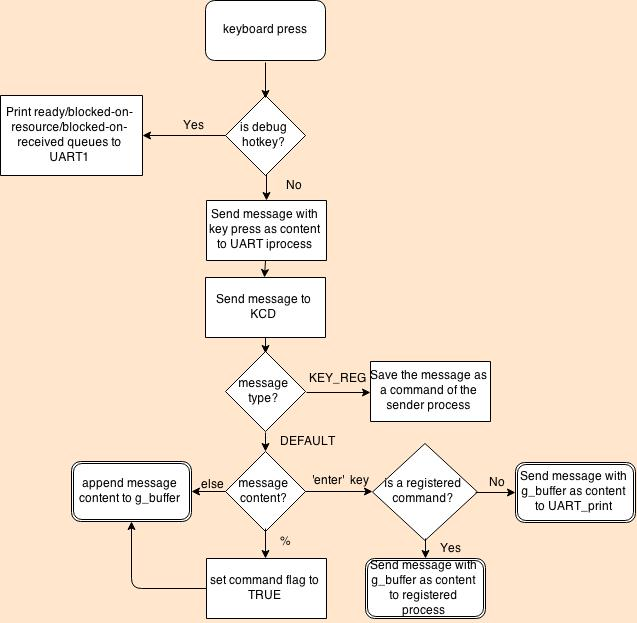
\includegraphics[width=150mm]{Keyboard_interrupt.jpg}
\caption{A Keyboard interrupt flowchart \label{overflow}}
\end{figure}

\section{Initialization}
The OS starts by initializing each of the interrupts (irq, timer, and uarts). Each of these are calls to given functions and were not implemented as part of this project and so will not be discussed in this report.

The OS then initializes the memory. This is done by setting the creating a pointer to the end of the available memory, \textbf{p\_end}. For each of the processes we move that pointer up by the size of a PCB to prevent them from being overwritten. A similar procedure is done for the ready, blocked on resource, blocked on received, and timed queues. The heap is now defined as starting at p\_end + 4 bits of buffer. The head end is defined as the end of available memory minus the amount of memory used for the stack of each process (RAM\_END\_ADDR - NUM\_PROCS - USR\_SZ\_STACK). At the start of this range the MSP is initialized, and within this range we create a Block with a null ownership pid and a next value pointing to the MSP. For each iteration we shift the MSP by BLOCK\_SIZE. This results in a heap of the appropriate bounds initialized as a linked list of BLOCK\_SIZE sized blocks.For more details view the associated section of 3.1.2.

Process initialization is done by building proc tables. The test processes are initialized using a \textbf{set\_test\_procs} function which builds a \textbf{g\_test\_procs} table with each of the test functions. Each function has default priority low and default stack size determined by a OS parameter \textbf{USR\_SZ\_STACK} We then set the starting values for A, B, and C to LOWEST. Finally each table entry is given a pointer to the corresponding function. When initializing all processes we call this set\_test\_procs function and iterate through the test table adding each entry to the \textbf{g\_proc\_table}. The rest of the functions are manually added since they have unique values. Most of these values are stored as global variables so that all functions have access to them. For more details view the associated section of 3.4.2

Parameters:
\begin{itemize}
    \item USR\_SZ\_STACK: the size of the stack allocated to each user process, this can be used to configure how much stack memory each process has access to
    \item RAM\_END\_ADDR: the ending address of available memory, this can be used to configure how much heap memory the OS has access (will be constrained by the hardware being used)
    \item BLOCK\_SIZE: the fixed size of each memory block, this can be used to configure the amount of memory given when request memory is called (can also be used to configure how many memory blocks to have)
\end{itemize}

\section{Testing}

\subsection{Test Handler}
Testing was done by creating a test handler that handled the set up, tear down, and printing of each test. The test handler was contained in \textit{usr\_proc.c} allowing test files to be separated and still use the handler. The test handler starts by printing the starting information, then it receives a message from each test and frees the memory used for that message. Once each of the five tests have finished the test handler is unblocked and it prints the ending information. A global variable is used to keep track of how many tests have failed to be printed.

\subsection{Test Procedure} Each test is initialized to LOW priority and the dummy test functions (A, B, and C) are initialized to LOWEST priority. When a test starts it sets its own priority and the property of any dummy tests that it uses to MEDIUM, this is done to ensure that only one test is running at a time in an isolated environment, ensuring that no tests interfere with each other. During its execution the test only messes with the priorities of the dummy test functions to keep this isolated state. Each test has a local variable \textbf{failed} which is used to count the number of internal assertions that have failed. Each test function also has a global counter (\textbf{function\_name\_count}) associated with it to allow assertions to be made between processes. When a test finishes it sets its priority to LOWEST and calls an endTest function. This function sends a message to the test handler, sets each of the dummy test functions and the test handler back to priority LOWEST, sets the global counters to 0, and checks the failed variable to print the correct output and update the global failed test counter. Essentially the endTest attempts to return everything to the same starting state and print the correct output at the end of each test.

\subsection{Part 1 Tests}
The part one tests focused on testing memory management and process priority switching (in \textit{usr\_proc1.c}).
\subsubsection{Test 1}
This test runs basic unit tests on getting and setting process priority. It starts with getting the priority of process A and checking that it is correct and that the appropriate ready queue contains A. It then tests preemption by setting process A to HIGH. Within A its global counter is incremented and the processor is released. This counter is checked to make sure that a did execute and return and the current priority of A is checked. This can also be con Finally the test attempts to set A to a invalid priority to ensure that an error is returned.
\subsubsection{Test 2}
This test runs basic unit tests on memory allocation and releasing. It starts by requesting a memory block and checking that the MSP has been updated appropriately. It then releases that memory block and checks that the MSP returns to the value it had initially. Next it checks the error codes by requesting a memory block, freeing it, then checking that the return value is RTX\_OK. The test then attempts to free the same memory block again and checks that the return value was RTX\_ERR.
\subsubsection{Test 3}
This test checks that memory ownership is enforced. It uses a global variable \textbf{test3\_mem} which is requested by test3. The test then sets B to MEDIUM and releases the processor. B then attempts to release test3\_mem, records the value in a global variable, and returns to test3. Test3 checks that B got a error when it attempted to release test3\_mem and releases it.
\subsubsection{Test 4}
This test checks what happens when we reach the end of memory. The test starts by requesting a bock of memory \textbf{test4\_mem}. This will be used later. The test then releases to C, Within test C we request exactly the number of free memory blocks +1. This should cause C to be blocked and the processor to switch back to test4. Here test4 checks that C has been put on the blocked on resource queue correctly. Then test4 releases the test4\_mem block which should trigger preemption back to C. Here C frees all of the memory that it allocated and returns to test4. Test4 checks that the amount of free memory blocks at the start of the test equals the amount of free memory at the end of the test to ensure that we have no memory leaks.
\subsubsection{Test 5}
This test focuses on ensuring that the way we manipulate our queues does not introduce memory leaks. We create generic queue elements containing two pointers (to the next element and to the data contained in the element). For efficiency we store multiple elements in a single memory block. Test5 starts by allocating enough elements to fill a memory block and checking that a new block has been allocated for them. It then released each of those elements and checks that the memory block allocated for them is returned correctly.

\subsection{Part 2 Tests}
The part two tests focused on testing message passing (in \textit{usr\_proc2.c}).

\textit{Note: the order of these tests seems a little odd, this is done to prevent tests from interfering with each other.}
\subsubsection{Test 1}
This test tests sending a receiving multiple messages. The test starts by sending a configurable number of messages to B (this value is stored in a variable NUM\_TEST\_MESSAGES\_MAILBOX) and checking that B's mailbox is of appropriate size. The test then switches to B who iterates through its mail box freeing each message, then returns to test1. This also tests that the special memory ownership related to message sending works since B is the one who releases the memory associated with the message.  This test can be used to evaluate the maximum number of messages the system can process at the same time.
\subsubsection{Test 2}
This test also tests sending and receiving multiple messages, but this test sends and receives one at a time instead of sending and receiving blocks of messages. The test records the number of free memory blocks then switches to B. Within a for loop of configurable size (stored in global variable NUM\_TEST\_MESSAGES) B creates a message, sends it, increments a counter (\textbf{messages\_sent}), and switches to test1. Within a similarly sized loop, test1 receives a message, deallocates it, increments a counter (\textbf{messages\_received}), and switches to B. Once the message sending is done we check that the ending number of free memory blocks is equal to the starting number of free memory blocks and that the number of messages sent is equal to the number of messages received. This ensures that there is no memory leak or lost messages. This test also runs the same procedure sending messages to itself. In theory this test can run for any number of messages.
\subsubsection{Test 3}
This test tests blocking and blocking from the blocked on receive queue. This test starts by immediately switching to C. C attempts to receive a message. It should be blocked and switch back to test3. Test3 checks that C is now on the blocked on receive queue then sends C a message and releases the processor. C should unblock, receive the message, increment a counter, and switch back to test3. Test3 checks the counter to make sure that C finished executing and checks that C has been removed from the blocked on receive queue.
\subsubsection{Test 4}
This test tests preemption on the blocked on receive queue. The test starts by setting A to HIGH priority which should preempt to A. A then attempts to receive a message and gets blocked with should preempt back to test4. Test 4 sends a message to A which should preempt back to A. A increments its counter and releases the processor. Then test4 just checks that A incremented its counter signifying that it finished running.
\subsubsection{Test 5}
This test contains the unit test for send, receive, and delayed send. The test starts by switching to A. A then sends two messages to test5, one with a delay and one without in that order (both messages contain different text to tell them apart), and releases the processor. Test5 now receives both messages. It checks that the sender was correctly sent and that the message text of the first message equal what we expect it to. It similarly checks that the text of the second message matches what should have been sent. This also ensures that the messages arrived in the correct order. Since the delayed message was sent first if it did not delay it would arrive first. We also watch the test to see that the test has the appropriate delay before printing.
\subsubsection{Manual Tests}
The Wall Clock was tested by manually entering each of the following commands after the automatic tests finished.

Manual tests:
\begin{itemize}
    \item \%W (wait a few seconds to watch it increment)
    \item \%WT
    \item \%W (wait a few seconds (check that the starting value is correct)
    \item \%WR (check that clock resets)
    \item \%WS 12:59:55 (watch to make sure it returns to 00:00:00)
    \item \%WS 33:00:00 (make sure that it does not set to invalid times)
    \item r (check that the ready queue is printed correctly)
    \item b (check that the blocked on resource queue is printed correctly)
    \item m (check that the blocked on receive queue is printed correctly)
    \item leave the wall clock running for a few minutes
\end{itemize}

\subsection{Part 3 Tests}
Part three is different from the other tests since it is implementing given pseudo code (in \textit{usr\_proc3.c}) with all other test process empty and uses a specialized test handler (in \textit{usr\_proc\_p3.c}). The automatic version of the test is simply the pseudo code listed in the assignment requirements.

Manual tests:
\begin{itemize}
     \item the above listed wall clock tests
     \item \%C 5 3 (move test4 to a new priority)
     \item r (check that test4 has changed priority)
     \item \%C 5 12 (check invalid priority)
     \item \%C 45 1 (check invalid process)
     \item \%C 10 3 (check forbidden processes)
     \item \%C 5 4 (check forbidden priority)
     \item \%C 8 0(check moving blocked processes)
 \end{itemize}

\subsection{Running the Tests} Tests were run automatically by the test handler (with the exceptions of the few listed manual tests). Each part's tests were contained in their own file separate from the test handler. To run a different set of tests we linked in that test file and ran it. Some exceptions were made for part 3 which required a different test handler due to its unique nature. Testing was done almost exclusively on the debugger, testing with the board only at the very end to make sure that the demo would run smoothly. This was done both to protect the board and allow us to the many tools built into the debugger.


\section{Major Design Changes}
Everyone
\begin{itemize}
\item What design decisions ended up being a mistake?
\item What were the major stumbling blocks?
\item What would you do differently if you started over?
\begin{itemize}
\item
Should have made a special i-process queue instead of putting in them in the ready queue with user processes
\item
Should not have i-processes depend on message passing. Instead, have the i-process block itself on finishing with input and be unblocked by the interrupt handler.
\end{itemize}
\item What design issues did your OS have?


\end{itemize}

\section{Timing Analysis}
Everyone

\section{Conclusion}
In hindsight, it is apparent that there are many implementation strategies which could have been drastically improved, saving hours of debugging and refactoring. However, with the spirit of the course, all contributors gained a deep understanding of the design and implementation challenges of basic operating systems, and can likely discuss the benefits and detriments of each decision that we made over the course of this project.

\end{document}
